% ========== Chapter 3
 
\chapter {\uppercase{A systems-level model of the microbial regulatory genome}}
\label{chap:3}

 Microbes can tailor transcriptional responses to diverse environmental challenges despite having streamlined genomes and a limited number of regulators. Here, we present data-driven models that capture the dynamic interplay of the environment and genome-encoded regulatory programs of two types of prokaryotes: \eco (a bacterium) and \halo (an archaeon). The models reveal how the genome-wide distributions of \textit{cis}-acting gene regulatory elements and the conditional influences of transcription factors at each of those elements encode programs for eliciting a wide array of environment-specific responses. We demonstrate how these programs partition transcriptional regulation of genes within regulons and operons to re-organize gene-gene functional associations in each environment. The models capture fitness-relevant co-regulation by different transcriptional control mechanisms acting across the entire genome, to define a generalized, system-level organizing principle for prokaryotic gene regulatory networks that goes well beyond existing paradigms of gene regulation.\\


 \noindent This chapter has been modified from:\\

\noindent Brooks AN$^{*}$, Reiss DJ$^{*}$, Allard A, Wu W, Salvanha DM, Plaisier CL, Chandrasekaran S, Pan M, Kaur A, Baliga NS. (2014) A system-level model for the microbial regulatory genome. \emph{Mol Syst Biol.}  10: 740.\\

 \noindent * Indicates equal contribution 

\paragraph{Chapter Highlights}

\begin{itemize}
\item Method to infer a genome-wide map of gene regulatory elements (GREs) and their 
condition-specific activities directly from genome sequence and transcriptome profiles
\item Novel co-regulatory structure, the \textbf{corem}, describes condition-specific partitioning 
and reorganization of operons and regulons by combinatorial and other nuanced regulatory mechanisms
\item Corems group together functionally related genes that have tight co-expression in 
some but not all environments
\item Corems associate genes from different operons and regulons that have highly similar 
fitness consequences
\end{itemize}


\section{Summary}
 
Genome-scale reconstruction of gene regulatory networks for two diverse microbial species using genome sequence and transcriptional profiles reveals complex, condition-dependent co-regulated modules (corems) and \textit{cis}-regulatory mechanisms that generate them. 

\section{Introduction}

Deciphering how microbes colonize dynamically changing environmental niches with few regulators and streamlined genomes will require mechanistic and system-level characterization of their gene regulatory networks (GRNs). Even a streamlined microbial genome encodes an intricate network of regulatory and signaling systems that sense and process extracellular and intracellular information to regulate gene expression at multiple levels (transcriptional, post-transcriptional, translational, allosteric, etc.). A significant fraction of these environmental signals are relayed by transcription factors (TFs) that modulate transcriptional activity when they bind DNA. TFs typically bind conserved, $\sim$6-20 nucleotide DNA sequences located in intergenic regions immediately adjacent to transcription initiation sites. These TF binding sites are referred to as gene regulatory elements (GREs). 

A goal of systems biology has been to map the complete set of TFs, GREs, and their interactions, using high throughput techniques including ChIP-chip \cite{blat_cohesins_1999}, yeast two-hybrid \cite{fields_novel_1989}, DNase I hypersensitivity \cite{crawford_identifying_2004}, or more modern variants using sequencing \cite{johnson_genome-wide_2007}. In parallel, attempts have been made to infer GRNs directly from gene expression data \cite{bonneau_predictive_2007,de_smet_advantages_2010,faith_large-scale_2007,segal_genome-wide_2003}. Such high throughput approaches are attractive because they would accelerate discovery in understudied organisms by circumventing significant labor and cost.

Inference of systems-scale GRNs that are both predictive and mechanistically accurate, however, has proven difficult for a number of reasons, including: (1) the statistical challenge of confidently discovering GREs across the genome, \textit{de novo}; (2) the consequences of non-linear gene regulatory dynamics, including combinatorial molecular interactions at gene promoters; and (3) the often non-canonical locations of GREs throughout the genome (including internal to operons and within coding sequences). A remaining challenge, therefore, is to produce an unbiased map of TF-binding site locations throughout the genome, including information about what binds to those sequences, in what contexts they are bound, and, importantly, how TF-binding throughout the genome ultimately influences cellular physiology.     

We previously constructed an ‘Environment and Gene Regulatory Influence Network’ (EGRIN) for \halo \cite{bonneau_predictive_2007}. This model was constructed in two steps. First, modular organization of gene regulation was deciphered through semi-supervised biclustering of gene expression, guided by biologically informative priors and \textit{de novo cis}-regulatory GRE detection for module assignment (cMonkey; \cite{reiss_integrated_2006}). Second, using a regression-based approach transcriptional changes of genes within each bicluster were modeled as a linear combination of influences of TFs and environmental factors (Inferelator; \cite{bonneau_inferelator:_2006}). 

The EGRIN networks learned by cMonkey and Inferelator accurately predicted transcriptional changes in new environments, a feat that has subsequently been replicated by other network inference strategies \cite{faith_large-scale_2007,lemmens_distiller:_2009,marbach_wisdom_2012}; yet, these network models have failed to capture detailed regulatory mechanisms that operate only in specific environments, at non-canonical genomic locations, or in complex combinatorial schemes. 

Here, we report significant advancement to inference of GRNs that overcomes many of these challenges. We have developed a methodology applicable to any sequenced microbe in culture to infer \egrine~models for two representative organisms from the primary branches of prokaryotic life - bacteria and archaea: (1) \eco, a bacterium with a wealth of information about transcriptional regulatory mechanisms and related experimental data \cite{salgado_regulondb_2006}; and (2) \halo, an archaeon with few examples of regulatory mechanisms that have been characterized in detail, but extensive experimental data from recently conducted systems biology studies \cite{bonneau_predictive_2007,koide_prevalence_2009}. The wide range of prior knowledge for these organisms proved invaluable for testing our model. In addition, we have also conducted new experiments that validate \egrine~predicted complex modulation of the \eco transcriptome structure during varying stages of growth in rich media. 

\egrine~models the organization of GREs within every promoter, their distributions across the entire genome – even in non-canonical locations – and links the contexts in which they act to conditional co-regulation of genes. These features are formalized in \egrine~by condition-specific, co-regulated modules or corems.  Corems are overlapping sets of co-regulated genes that, in some cases, group together genes from different regulons and, in other cases, subdivide genes of the same regulon, or even the same operon. \egrine~formalizes how the genome-wide coordination of previously characterized and newly discovered regulatory mechanisms dynamically associates genes into corems, bringing together functionally-related genes from different operons and regulons whose deletions have similar impact on cellular fitness. Our results show how prokaryotes, much like eukaryotes, can produce complex gene expression patterns with a relatively small number of regulatory components.  

\section{Results}

\subsection{Construction of \egrine} 

We developed an ensemble-framework that models the condition-specific global transcriptional state of the cell as a function of combinations of transient TF-based control mechanisms acting at intergenic and intragenic promoters across the entire genome. Specifically, for each of the two orgainsms, \halo and \eco, we aggregated associations across genes, GREs, and environments from many individual EGRIN models, each trained on a subset of the gene expression data, to (1) quantify confidence in each model-predicted association; (2) reveal context-dependent regulatory mechanisms that occur infrequently in the data; and (3) discover non-canonical regulatory mechanisms. We refer to the aggregated, post-processed ensemble of EGRIN models as \egrine, and conditionally co-regulated modules as corems (details provided in Chapter \ref{chap:2}, Figure \ref{fig:egrin2:1}; ensemble statistics available in Table \ref{tab:stats}). 

\begin{figure}[h!]
    \centering
    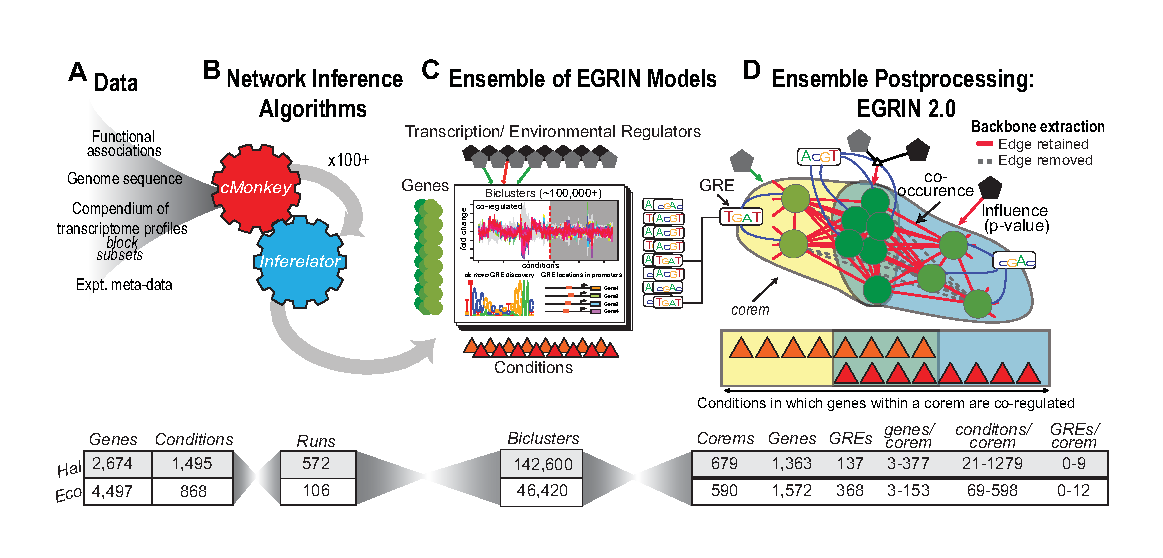
\includegraphics[width=0.9\textwidth]{figures/egrin2_fig1}
 	\caption[\egrine~Model Construction.]{\egrine~Model Construction. Workflow summary for \egrine. Tables below each panel contain detailed statistics for the \halo and \eco models. (A) and (B). The cMonkey and Inferelator algorithms were applied many times to subsets of gene expression data from large compendiums of transcriptome profiles to construct many individual EGRIN models.(C) Individual EGRIN models were integrated into an ensemble for filtering, querying, and ranking relationships among genes (circles), regulators (hexagons), motifs (sequence logos), and the conditions (triangles) in which these relationships were discovered.(D) The library of relationships was mined using algorithms for motif clustering, backbone extraction, and community detection to construct the final \egrine~model. In \egrine, overlapping co-regulated sets of genes (corems, shaded regions of the graph) are statistically associated with specific gene regulatory elements (GREs, sequence logos, blue edges), regulatory influences (pentagons, green or red depending on direction), and environments in which they are co-regulated (triangles). Each node represents a gene in the model. Genes are connected via co-regulation edges, with weights that reflect the number of occurrences in the ensemble. Dashed edges were removed from the model by backbone extraction.}
    \label{fig:egrin2:1}
\end{figure}

\subsection{\egrine~discovers experimentally characterized regulatory mechanisms}

A high quality GRN has to be both comprehensive (high recall) and accurate (high precision). To evaluate the quality of \egrine, we compared its predictions on \eco to RegulonDB \cite{gama-castro_regulondb_2011}, an extensive, manually-curated, gold-standard of experimentally validated TF-gene interactions. We compared the genome-wide distribution of each \textit{de novo} discovered GRE in \egrine~to experimentally characterized binding locations of every TF in RegulonDB. This comparison showed that \egrine~had accurately located binding sites for 60\% of experimentally characterized TFs in RegulonDB (53 out of 88 at FDR $\leq$ 0.05 for all TFs with $\geq$3 unique sites; see Chapter \ref{chap:2}). At a standard precision cutoff of 25\%, \egrine~recovered 577 ``strong evidence'' TF-gene interactions, which is 2.7X as many validated interactions as algorithms that exclusively use expression data, i.e. without genomic sequence information (Figure \ref{fig:egrin2:2:A}, Figure \ref{fig:pr_curves}, Figure \ref{fig:cumulative_auprs}, Figure \ref{fig:argR_purR_networks}, Table S4, \ref{chap:2}; \cite{faith_large-scale_2007,marbach_wisdom_2012}. As expected, the ensemble network had greater precision and recall than individual cMonkey runs. Furthermore, integration of Inferelator-predicted TF influences with GRE-based predictions increased overall algorithm performance. These results show that integrating complementary methods, such as regression-based inference of TF regulation, biclustering-based inference of network modularity, and \textit{de novo} GRE detection, improves the accuracy and coverage of the inferred GRN. 

\begin{figure}[h!]
    \centering
    \includegraphics[width=0.75\textwidth]{figures/egrin2_AUPR}
 	\caption[\egrine~Model Validation: Performance on RegulonDB]{\egrine~performance on experimentally-validated gold-standard network. Comparison of \egrine~model components (“GRE”: GRE-only; “Inf”: Inferelator-only) to the DREAM5 community ensemble network, against RegulonDB (strong evidence code). (Top) Area under the precision-recall curve (AUPR) and (Bottom) number of correct predictions at 10, 25, and 50\% precision. 
}
    \label{fig:egrin2:2:A}
\end{figure}

Since few GREs have been characterized in \halo, we performed a global assessment and discovered that GREs in \egrine~occur at consistent locations across many gene promoters throughout the genome (Figure \ref{fig:gre_global_locs_hal}). We could even assign putative roles for some GREs based on their location relative to transcription start sites (TSSs). For instance, the location of TATA box-like elements (GRE \#25) between -21 to -40 nucleotides upstream of TSSs in \halo is consistent with the characterized location of basal elements in archaeal promoters (TFB/TBP complex recognition sites) \cite{geiduschek_archaeal_2005}. Similarly, other elements occurred either consistently downstream of the TATA box (putative repressors, e.g. GRE \#1 and \#2) or upstream of these basal elements (putative activators, e.g. GRE \#5). Thus, even in organisms where genome-wide TF binding data are scarce, \egrine~can be used to infer and predict putative roles for \textit{de novo} discovered GREs.

\subsection{Corems model genes with similar effects on organismal fitness}

We investigated whether the model goes beyond simple co-expression to group together genes that have similar phenotypic contributions. We did this because previous studies have reported weak correlation between gene expression and fitness \cite{price_indirect_2013}. For all genes in each corem, we computed pairwise correlations of fitness effects in a dataset generated from a survey of relative growth rates for 3,902 single gene deletion strains of \eco subjected to a chemical genomics screen spanning 324 different environmental conditions \cite{nichols_phenotypic_2011}. We discovered that more than one-third of gene-pairs with the most similar fitness effects across environments (Pearson correlation $>$ 0.75) were grouped together in corems. We evaluated significance of this result by performing similar analysis using modules based-on co-expression (WGCNA; \cite{langfelder_wgcna:_2008}), and regulons (RegPrecise and RegulonDB), where a regulon is defined as a set of genes regulated by the same TF. While WGCNA and regulons also grouped significant numbers of high fitness-correlated gene-pairs (one-sided KS-test $<$ 0.05), corems were more enriched for highly similar fitness associations (higher KS D-statistic) and in general provided greater precision and coverage (Figure \ref{fig:egrin2:2:B}). As an example, corems group together 5X as many gene-pairs with highly correlated fitness effects as RegPrecise, RegulonDB, or WGCNA (134 out of 185 gene-pairs with Pearson correlation ≥0.9 are discovered in corems, Table S5). Most important, corems retained a high degree of enrichment for gene-pairs with highly correlated fitness effects after removing all associations attributable to operon and regulon memberships, and even combinatorial control (Figure \ref{fig:fitness_wo_operons}, Table S5\footnote{All tables available in \cite{brooks_systemlevel_2014} and \href{http://egrin2.systemsbiology.net}{online}}). This suggested that corems model regulatory associations among genes that cannot be explained within the existing paradigms of regulons and operons. 

\begin{figure}[h!]
    \centering
    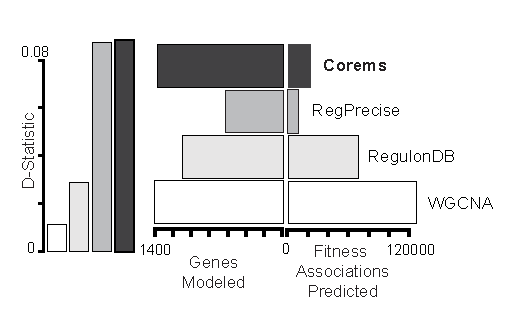
\includegraphics[width=0.75\textwidth]{figures/egrin2_corem_fitness}
 	\caption[\egrine~Model Validation: Fitness contributions]{Enrichment of similar fitness effects within gene modules. (Left) Magnitude of enrichment for gene pairs with similar fitness consequences, assessed by one-tailed KS-test (KS D-statistic). (Right) Number of genes and gene-pairs predicted by each method.  Comparison methods include \egrine~corems, co-expression modules from WGCNA, and regulons from databases (RegPrecise and RegulonDB). 
}
    \label{fig:egrin2:2:B}
\end{figure}

In other words, corems group together genes that are regulated by distinct TFs. For example, the ArgR-regulated acetylglutamate kinase, \textit{argB}, and \textit{ilvC}, an IlvY-regulated ketol-acid reductoisomerase have fitness correlation of 0.95 (Pearson coefficient), which suggests an important coupling between branched-chain amino acid biosynthesis and arginine metabolism (Table \ref{tab:table1}). Although these genes are regulated by distinct TFs (ArgR and IlvY, respectively), the high similarity of their expression changes across multiple environments brings them together into the same corem (ec512157). There are 319 highly correlated (Pearson correlation $\geq$ 0.75) fitness associations among genes from different regulons that are modeled by corems – each of which suggests an important physiological coupling that results from the coordinated activity of TFs (Table E6). These examples illustrate how the organizing principle of corems captures fitness-relevant associations within a GRN that are overlooked by current definitions for gene-gene co-regulation, such as regulon and operon.

\subsection{\egrine~predicts detailed organization and context-specific importance of GREs in gene promoters}

We next investigated accuracy of \egrine~predicted spatial organization of GREs, and their context-specific roles in mediating transcriptional regulation from specific promoters. We did this analysis in context of one of the best studied \halo promoters: \textit{kdpFABC}, with data not used for model training. The \textit{kdp} operon encodes an ATP-dependent potassium transporter that counterbalances extremely high salinity in the extracellular environment. \egrine~predicts that at least three GREs are putatively responsible for mediating transcriptional regulation of this operon: GRE \#1, GRE \#148, and GRE \#106 (Figure \ref{fig:egrin2:2:C}). The locations of these GREs align to regions that were experimentally characterized in an independent study as “Operator” and “BRE-TATA” elements, respectively. This demonstrates that \egrine~is able to accurately predict the organization of GREs in gene promoters at nucleotide-resolution.

\begin{figure}[h!]
    \centering
    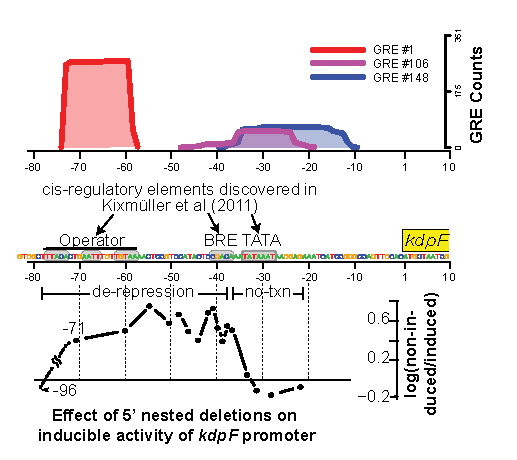
\includegraphics[width=0.75\textwidth]{figures/egrin2_kdpvalidaton}
 	\caption[\egrine~Model Validation: Regulatory elements of \textit{kdp} operon, \halo]{Promoter architecture of the \halo \textit{kdpFABC} promoter predicted by the \egrine~model. (Top) Frequency of GRE alignment to each position in the \textit{kdpFABC} promoter. GREs are indicated by shaded lines. (Middle) Genome sequence marked with putative functions by \cite{kixmller_archaeal_2011}. (Bottom) Transcriptional activity measurements from truncated promoters used by authors to validate these sites. 
}
    \label{fig:egrin2:2:C}
\end{figure}

Since these sites also had characterized transcriptional roles [determined by promoter truncation experiments \cite{kixmller_archaeal_2011}], we asked whether \egrine~would have been able to predict these roles given the context in which the GREs were discovered. Strikingly, we find that GRE \#1 (aligned to the “Operator”) was discovered in environments, including low salt (hypergeometric FDR = $6.9\times10^{-12}$), where the transcript is repressed (one-sided t-test pval = 0.048), while GRE \#106, which aligns to the “BRE-TATA” region, was discovered in environments, including low oxygen (hypergeometric FDR = $1.8\times10^{-9}$), where transcript levels are elevated (one-sided t-test pval = $1.2\times10^{-3}$; \ref{chap:2}). Here onwards, we will refer to a GRE as ``active'' when it is predicted to be important for transcriptional regulation at a specific promoter (see Figure \ref{fig:corem_gres} for details). The environmental contexts in which the three GREs in the \textit{kdp} promoter are predicted to be active are especially interesting because perturbations to external potassium levels and energy-producing mechanisms have been shown to significantly influence expression of this operon \cite{wurtmann_evolutionarily_2014}. Thus, \egrine~had accurately predicted that a trade-off in relative influence of GRE \#1 (repressing) versus GRE\#106 (activating) controls expression levels of this operon in a condition-specific manner, exactly as was characterized by independently performed experiments. This is powerful because it shows that using \egrine~we can predict when (context) and how (activate or repress) a specific GRE(s) within a promoter might act, even though we might not know the precise regulatory mechanism (e.g., TF binding/unbinding, allosteric activation, co-factor interaction, etc).

\subsection{Conditionally active GREs within each promoter reorganize gene memberships within corems}

We investigated whether \egrine~accurately links the same GRE at different promoter locations, the environments in which it is predicted to be active within each of those promoters, and conditional co-regulation of the associated genes (see \ref{chap:2}). We did this analysis with genes of nucleotide biosynthesis in \eco, including key branch-point enzymes \textit{carA} (\textit{b0032}) and \textit{pyrL} (\textit{b4246}), since they are canonical, extremely well studied pathways that are critical for survival. Regulation of \textit{carA}, which catalyzes synthesis of an important metabolic intermediate in several amino acid and nucleotide metabolism pathways (carbamoyl phosphate), is known to be sensitive to purine and pyrimidine pools, as well as arginine \cite{neidhardt_escherichia_1996}. \egrine~discovered several previously characterized and new mechanisms for regulation of carA, including two GREs (GRE \#4 and GRE \#12) that match to consensus sequence motifs for PurR and ArgR, respectively \cite{piette_dna_1984} (Figure \ref{fig:egrin2:2:D}). Remarkably, \egrine~discovered novel overlapping organization of GRE \#4 and GRE \#12 in the \textit{pyrL} promoter that was not previously reported in RegulonDB (Figure \ref{fig:pyrL}). This promoter organization was verified upon mapping overlapping binding sites for ArgR and PurR precisely at the predicted locations in ChIP-chip data that were not used in model training \cite{cho_deciphering_2012,cho_purr_2011}.

\begin{figure}[h!]
    \centering
    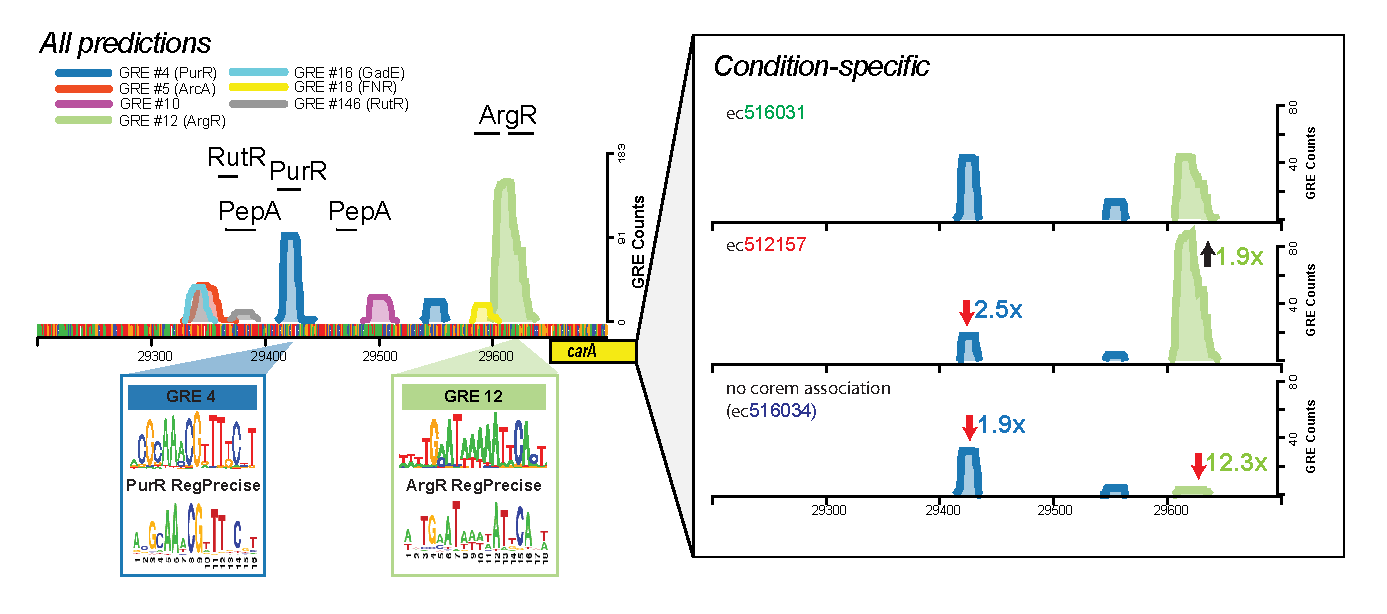
\includegraphics[width=\textwidth]{figures/egrin2_carA}
 	\caption[\egrine~Model Validation: Regulatory elements of \textit{carA}, \eco]{Predicted architecture of the \eco \textit{carA} promoter across all ensemble predictions (as in Figure \ref{fig:egrin2:2:C}). Horizontal bars above peaks mark experimentally characterized TF binding sites (RegulonDB). Significant GRE matches to characterized \eco binding sites in RegulonDB are indicated in parentheses. (Right) Condition-specific states of the \textit{carA} promoter. Variation in conditional discovery of GREs (counts and fold-change relative to ec516031, top) suggests when they are “active” across three different subsets of experimental conditions in the carA promoter. (Bottom). Condition subsets correspond to co-regulation of \textit{carA} with genes in the nucleotide and pyrimidine corems (ec516031, ec512157) or environments where \textit{carA} is not co-regulated with genes in any corem (ec516034). Motif logos for GRE \#4 (PurR) and GRE \#12 (ArgR) from the \egrine~predictions compared to logos from RegPrecise. 

}
    \label{fig:egrin2:2:D}
\end{figure}

\begin{figure}[h!]
    \centering
    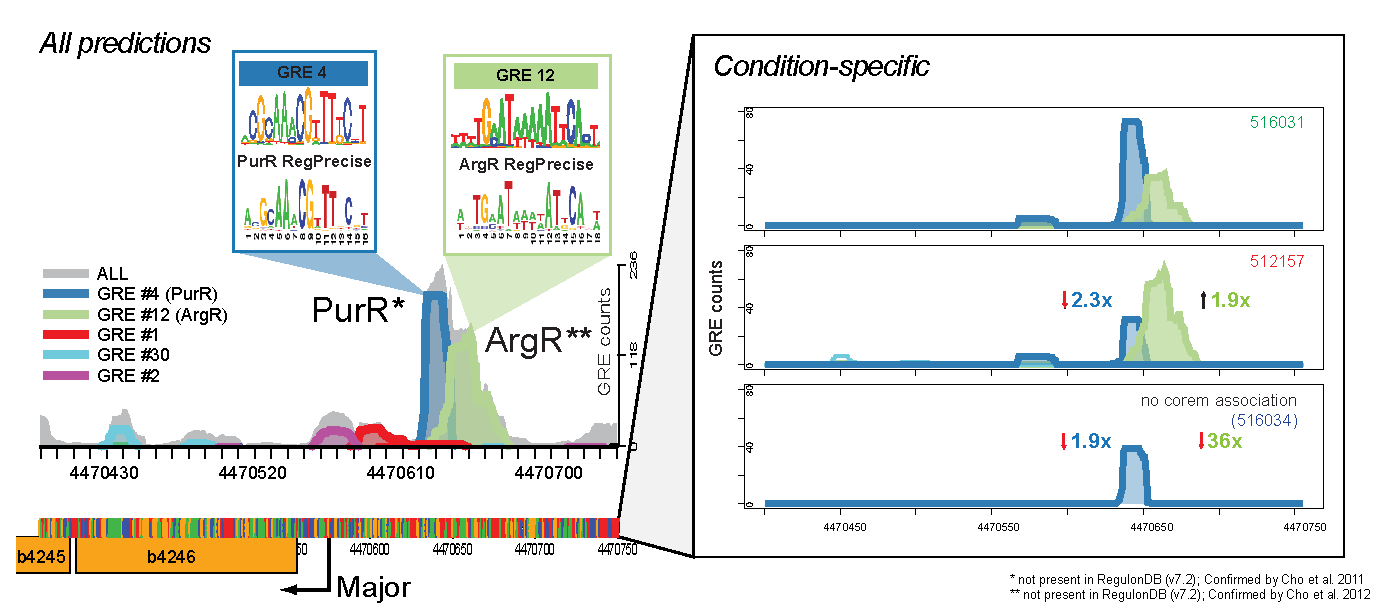
\includegraphics[width=\textwidth]{figures/pyrL}
 	\caption[\egrine~Model Validation: Regulatory elements of \textit{pyrL}, \eco]{Differential GRE activity in \textit{pyrL} promoter, \textit{E. coli}. (Left) Predicted promoter architecture for \textit{E. coli pyrL} (b4246). Overlapping GREs matching to PurR (GRE \#4) and ArgR (GRE \#12) were detected upstream of \textit{pyrL}. These sites were not annotated in RegulonDB, but were validated in independent ChIP-chip experiments \cite{cho_purr_2011,cho_deciphering_2012}. Transcription start site indicated with arrow. (Right) Condition-specific promoter architectures for \textit{E. coli pyrL} (as in Figure \ref{fig:egrin2:2:D}). Variation in predicted GRE activity across three different subsets of experimental conditions (counts and fold-change) for two GREs in the \textit{pyrL} promoter. Experimental subsets correspond to conditions under which at least one of three nucleotide biosynthetic corems is regulated (denoted by colored names at top-right of each plot)
}
    \label{fig:pyrL}
\end{figure}

We were most interested, however, to understand the consequences of conditional regulation at ArgR and PurR-associated GREs on variable expression of \textit{carA} in different environments. Indeed, \egrine~predicts three condition-specific states of the \textit{carA} promoter with respect to when PurR- and ArgR-matched GREs are conditionally active: (1) high PurR and high ArgR, (2) low PurR and high ArgR, and (3) high PurR and low ArgR (Figure \ref{fig:egrin2:2:D}). Interestingly, two of these promoter states correspond to co-regulation of \textit{carA} with a different combination of genes (i.e., different corems), functionally separating pyrimidine from purine biosynthesis (Figure \ref{fig:egrin2:4:B}), while the third state is not associated with co-regulation of \textit{carA} with the genes of any corem. Thus, the context in which GREs are active accurately explains when and how genes are co-regulated in different overlapping combinations to perform distinct functions.

\subsection{Conditionally active GREs within operons generate multiple, overlapping, and differentially regulated transcript isoforms}

Some of the GREs discovered in \egrine~occur in non-canonical locations and lead to unexpected transcriptional behaviors, such as the subdivision of operons into multiple transcriptional units.  Previously, we reported pervasive modulation of the \halo transcriptome structure by transcriptional elements that are located within operons and coding regions \cite{koide_prevalence_2009}. \egrine~recapitulated this phenomenon by sub-dividing operon genes into different corems. In all, the model predicted that nearly one-third of all \halo operons generate multiple transcript isoforms (Figure \ref{fig:nirH}, Figure \ref{fig:sdh},Figure \ref{fig:vng2211h}, Chapter \ref{chap:2} for details). Nearly half of these predictions of conditional operon structures were corroborated by experimentally mapped transcriptional breaks (hypergeometric pval = $4.2\times10^{-3}$; Table S7; Koide et al., 2009). Often, these transcript boundaries were adjacent to GREs that coincide with experimentally determined TFB-binding sites (\cite{facciotti_general_2007}; Figure \ref{fig:egrin2:3:A}), reinforcing the accuracy of \egrine~predictions.

\begin{figure}[h!]
    \centering
    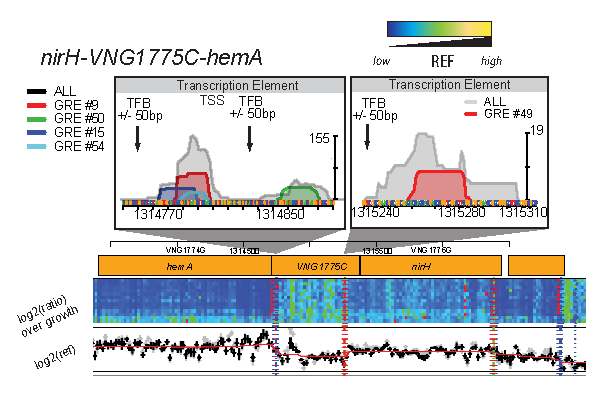
\includegraphics[width=0.75\textwidth]{figures/nirH}
 	\caption[Transcriptional evidence for multiple transcript isoforms from the same operon: \textit{nirH-VNG1775C-hemA}, \halo ]{GREs regulate multiple transcript isoforms from operons in \textit{H. salinarum, nirH-VNG1775C-hemA}. GREs located inside operons coincide with experimentally measured transcriptional break sites. Experimentally determined tran- scription break sites (red dashed lines) above expression profiles of these regions across growth (heatmap \cite{koide_prevalence_2009} and ChIP-chip TFBs \cite{facciotti_general_2007}, vertical arrows) support the role of GREs in regulating segmentation of the operon in certain conditions. Insets contain regions immediately surrounding transcriptional break sites, including counts of GREs discovered at these locations.
}
    \label{fig:nirH}
\end{figure}

\begin{figure}[h!]
    \centering
    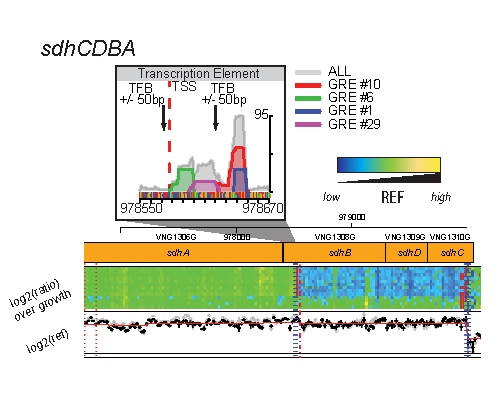
\includegraphics[width=0.75\textwidth]{figures/sdh}
 	\caption[Transcriptional evidence for multiple transcript isoforms from the same operon: \textit{sdhCDBA}, \halo ]{GREs regulate multiple transcript isoforms from operons in \textit{H. salinarum, sdhCDBA}. Caption details included in Figure \ref{fig:nirH}.}
    \label{fig:sdh}
\end{figure}

\begin{figure}[h!]
    \centering
    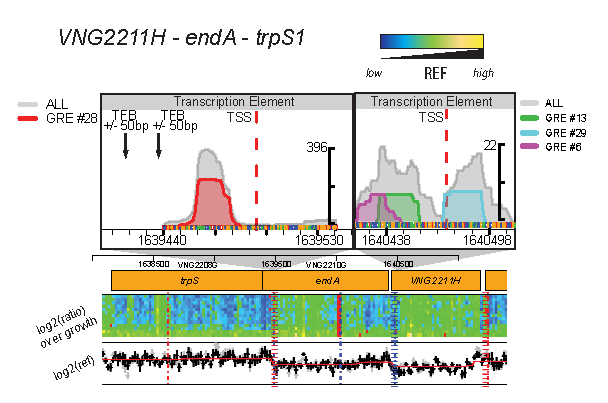
\includegraphics[width=0.75\textwidth]{figures/vng2211h}
 	\caption[Transcriptional evidence for multiple transcript isoforms from the same operon: \textit{VNG2211H-endA-trpS1}, \halo ]{GREs regulate multiple transcript isoforms from operons in \textit{H. salinarum, VNG2211H-endA-trpS1}. Caption details included in Figure \ref{fig:nirH}.}
    \label{fig:vng2211h}
\end{figure}

\begin{figure}[h!]
    \centering
    \includegraphics[width=0.8\textwidth]{figures/egrin2_dpp_1}
 	\caption[Transcriptional evidence for multiple transcript isoforms from the same operon, \halo ]{(Top) Predicted GREs located within (left) and upstream of (right) the \halo \textit{dpp} operon. Locations of experimentally mapped TFB binding sites (vertical arrows; \cite{facciotti_general_2007}), and experimentally mapped transcription break sites (vertical red dashed lines, see (B); \cite{koide_prevalence_2009}) are indicated. Locations of predicted GREs relative to coding segments of the \textit{dpp} operon. (Midlle) Expression changes during growth in the genomic region covering the \textit{dpp} operon measured by high-resolution tiling microarray. Raw RNA hybridization signal from mid-log growth phase indicated below. (Bottom) Three predicted transcripts from the \textit{dpp} operon. Internal colors correspond to the GREs putatively responsible for regulating each transcript (shown at top, derived from corem membership in Figure \ref{fig:egrin2:3:B}). Boxed colors indicate corem membership for each transcript (described in Figure \ref{fig:egrin2:3:B}). Red dashed lines indicate experimentally measured transcription break sites. Transcriptional break at lag phase highlighted by an arrow. Functional annotation for each gene located at bottom.
}
    \label{fig:egrin2:3:A}
\end{figure}

We further investigated whether \egrine~provides insight into downstream consequences of differentially regulating multiple transcript isoforms from the same operon. The \textit{dppAB1C2-oppD2-ykfD-VNG2342H} operon (hereafter the ‘\textit{dpp} operon’) in \halo encodes an ATP-dependent dipeptide transporter. Some periplasmic binding proteins (like \textit{dppA}) have the reported ability to function in conjunction with different ABC transport systems, giving support to the hypothesis that \textit{dppA} can be regulated independently \cite{higgins_binding_1990}. Despite high co-expression of the entire operon in the training data (mean R$^{2}$ = 0.6 across 1495 conditions), \egrine~predicted that the genes of this operon are transcribed as three different isoforms, each co-regulated with genes of a different corem: (1) the entire operon (hc21645 –“\textit{dpp} corem”), (2) the entire operon except the leader gene, \textit{dppA} (hc21279 –“permease corem”), and (3) just \textit{dppA} (hc6326 –“leader corem”). These predicted isoforms were verified by experimentally mapped transcript boundaries (Figure \ref{fig:egrin2:3:B}). Each of these corems contains a different dpp isoform and is enriched for a different biological function, including vitamin biosynthesis, porphyrin metabolism, and purine biosynthesis, respectively (Figure \ref{fig:egrin2:3:B}). Predicted differential regulation of the core permease (\textit{dppB1C2-oppD2-ykfD-VNG2342H}) with porphyrin metabolism genes in the permease corem is consistent with the reported capability of this transporter system to uptake heme when it functions with a different solute binding protein (i.e., without \textit{dppA}; \cite{letoffe_housekeeping_2006}). Overall, \egrine~provided insight into the distinct environment-dependent functional associations of each transcript isoform.   

Further, \egrine~revealed that segmentation of the \textit{dpp} operon into multiple corems is mediated by conditionally active GREs located both upstream and internal to the operon. For example, \egrine~predicted that GRE \#6 was responsible for disassociating \textit{dppA} transcription from the remainder of the operon. Interestingly, GRE \#6 was also discovered in the promoters of nearly all of the other genes in the leader corem (Figure \ref{fig:egrin2:3:A}, Figure \ref{fig:dpp_networks}, Table S8). Similarly, GRE \#1 was implicated in co-regulating the permease-encoding transcript with other genes in the permease corem, and GRE \#17 for co-regulating the entire operon with other genes in the \textit{dpp} corem. \egrine~ also predicted specific segmentation pattern of the dpp-operon during ‘lag growth phase’. This prediction was verified upon observing that a transcript break appears downstream to \textit{dppB1} precisely when a batch culture transitions from lag to log phase of growth (indicated by arrow in Figure \ref{fig:egrin2:3:A} heatmap). This is just one of 98 operons with experimentally validated conditional isoforms in \halo. For each instance, a similar correspondence between mechanism, context, and function could be demonstrated (Figure \ref{fig:nirH}, Figure \ref{fig:sdh},Figure \ref{fig:vng2211h}, and online).   Interestingly, even in \eco, where previous studies report a single transcript for the \textit{dpp} operon \cite{abouhamad_dipeptide_1994}, \egrine~ discovered that it is actually transcribed as multiple, condition-specific transcript isoforms, each of which participates in a different physiological process (Figure E5A).

\begin{figure}[h!]
    \centering
    \includegraphics[width=0.65\textwidth]{figures/egrin2_dpp_2}
 	\caption[Functional consequences of multiple transcript isoforms from the same operon, \halo]{ (Left) Three \halo corems model differential regulation of \textit{dpp} operon isoforms: (1) the entire operon (hc21645 –“\textit{dpp} corem”; top); (2) five tail genes, excluding \textit{dppA} (hc21279 –“permease corem”; center); and (3) the leader gene, \textit{dppA} (hc6326 –“leader corem”; bottom). Colored numbers denote quantity of genes in each corem; numbers in black shaded circles indicate the number of genes shared between corems. Pie charts represent average predicted influence of GREs on regulation of genes in each corem (see Figure E3B for detail). (Top-Right) Pie chart key indicates GRE identity. (Bottom-Right) Tables list enriched gene functions \cite{dennis_david:_2003} and environmental conditions for each of the corems (computed using the environmental ontology; see Chapter \ref{chap:2})
}
    \label{fig:egrin2:3:B}
\end{figure}

\begin{figure}[h!]
    \centering
    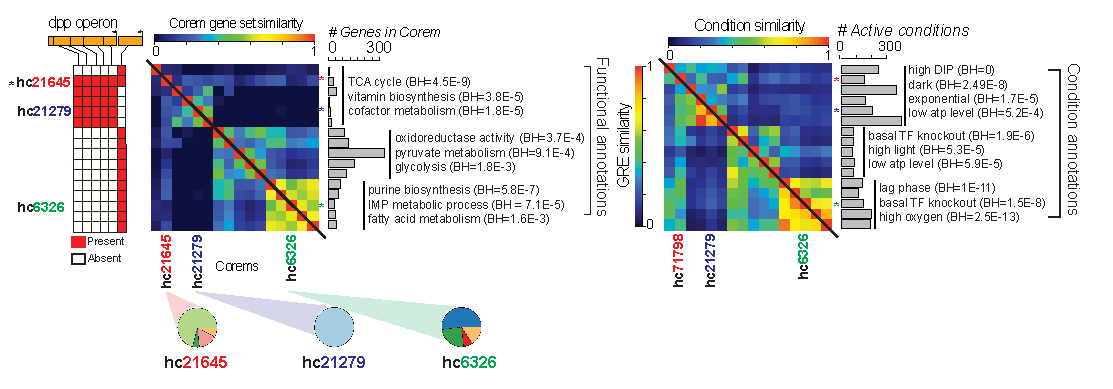
\includegraphics[width=\textwidth]{figures/dpp_heatmaps}
 	\caption[Alternate regulatory modes for \textit{dpp} operon predicted by corems, \halo]{Corems group together functionally related sets of genes that are co-regulated in similar environments by similar factors (Left) Presence/absence of \textit{dpp} operon genes in corems. Three classes of corems exist for the dpp operon: (1) the entire operon (e.g.hc21645), (2) the leader gene dppA (e.g.hc6326), and (3) five ``tail'' genes excluding \textit{dppA} (hc21279). (Middle) Gene similarity between corems (heatmap, Jaccard index). Functional annotations of genes in three highly similar clusters of corems to right. GRE composition for three corems shown below (pie chart, see Figure \ref{fig:corem_gres}). (Right). Similarity of conditions regulated (heatmap, upper triangle, Jaccard index) and GREs (heatmap, lower triangle, Jaccard index) among corems. Ordering is identical to (Middle). Environmental Ontology term enrichment (see Chapter \ref{chap:2}) for three clusters depicted to right.
}
    \label{fig:dpp_heatmaps}
\end{figure}

\begin{figure}[h!]
    \centering
    \includegraphics[width=0.75\textwidth]{figures/dpp_networks}
 	\caption[Network representation of transcriptional isoforms for the \textit{dpp} operon predicted by corems, \halo]{Network representation of transcriptional isoforms for the \textit{dpp} operon predicted by corems. Genes represented by circles. Edge colors and colored region behind the network indicate corem membership. Pie charts reflect GRE composition of each gene (see Figure \ref{fig:corem_gres}). Key for pie charts at top. Shading behind nodes (center of network) indicates dpp operon genes.
}
    \label{fig:dpp_networks}
\end{figure}

\begin{figure}[h!]
    \centering
    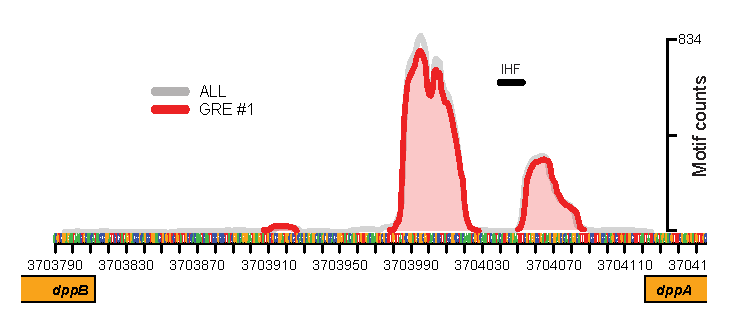
\includegraphics[width=0.75\textwidth]{figures/dpp_ecoli}
 	\caption[Evidence for condition-specific transcript isoforms of the \textit{dpp} operon in \textit{E. coli}]{EGRIN 2.0 predicts conditional modulation of \textit{dpp} operon in \textit{E. coli} as well. Promoter architecture within intergenic space between \textit{dppA} and \textit{dppB} suggested locations for TF binding internal to the operon (as in Figure \ref{fig:egrin2:3:A}). GRE binding sites are proximal to an experimentally characterized IHF binding site (black horizontal bar; RegulonDB).
}
    \label{fig:dpp_ecoli}
\end{figure}

While we were aware of extensive transcriptional heterogeneity within operons in \halo, we were surprised that \egrine~ predicted that the same phenomenon also occurred extensively in \eco. To see if this were true, we mapped the \eco global transcriptome structure across varying phases of growth in rich media using a densely tiled microarray (see Chapter \ref{chap:2}). We used this new gene expression data set to identify the corems in which different combinations of operon genes (i.e., transcript isoforms) were co-regulated in some or all phases of growth, and to characterize transcriptional breaks using previously developed methodologies \cite{koide_prevalence_2009}. We observed transcriptional breaks in nearly 20 percent of operons (including the \eco \textit{dpp} operon) just over this 9-time point growth study, validating \egrine~ prediction that nearly one-quarter of all \eco operons have conditional isoforms during varying stages of growth (hypergeometric pval = $1.07\times10^{-5}$, Figure \ref{fig:dpp_ecoli_expression}, Figure \ref{fig:galE}, Figure \ref{fig:ptsh}, Table S7). Experimental validation of this enormous transcriptional heterogeneity among operons in \eco demonstrates the power of \egrine~ to distinguish nuanced patterns in complex data, and provide both mechanistic explanation and context for when and why the novel phenomena might occur.

\subsection{Some TFs act similarly across certain environments to co-regulate functionally-related subsets of genes across their respective regulons}

We investigated whether \egrine~ provides insights into context-dependent  differential regulation of branched metabolic pathways – even those that have been meticulously studied for decades, such as \textit{de novo} biosynthesis of nucleotides in \eco \cite{neidhardt_escherichia_1996}. At least seven GREs were implicated in partitioning (purine biosynthesis: ec516034 –“purine corem”; pyrimidine biosynthesis: ec512157 –“pyrimidine corem”) or co-regulating (ec516031 –“nucleotide corem”) nucleotide biosynthesis into multiple overlapping corems (Figure \ref{fig:egrin2:4:A}, Figure \ref{fig:purR_heatmap}, Figure \ref{fig:purR_network}). The genome-wide locations for four of these GREs significantly overlapped with known binding locations for PurR, ArgR, MetJ, and IclR. Partitioning and co-regulation of purine and pyrimidine biosynthesis can be attributed to the location of these GREs in promoters of pathway genes, including \textit{carA}, and the environments in which they are predicted to be active (Figure \ref{fig:egrin2:2:D}). \egrine~ predicts, for example, that MetJ (GREs \#19, \#87) acts in conjunction with PurR (GRE \#4) to differentially regulate genes specific to the pyrimidine biosynthetic branch (pyrimidine corem), while (yet to be identified) TFs that bind GREs \#2 and \#206 function with PurR (GRE \#4) to regulate genes in the purine branch (purine corem) (Figure \ref{fig:egrin2:4:B}). The organization of these GREs within and across promoters, and the environments in which they act to mediate regulation by specific TFs, generates complex co-expression patterns among different combinations of genes in the three corems of this highly canalized pathway (filled violin plots, Figure \ref{fig:egrin2:4:C}). These conditional co-expression patterns predict that in certain environments the two branches are differentially regulated, while in others they are co-regulated as one unit. Consistent with this observation, fitness consequences of deleting genes in these corems vary across conditions (Figure \ref{fig:egrin2:4:D}, Figure \ref{fig:purR_corem_fitness}, Figure \ref{fig:purR_corem_fitness_specific}). For instance, knockouts of genes in all three corems have similar consequences on fitness in the presence of glucose. By contrast, in the presence of the toxic ionophore carbonyl cyanide m-chlorophenyl hydrazone (CCCP), only knockouts of genes in the nucleotide corem significantly alter fitness.

\begin{figure}[h!]
    \centering
    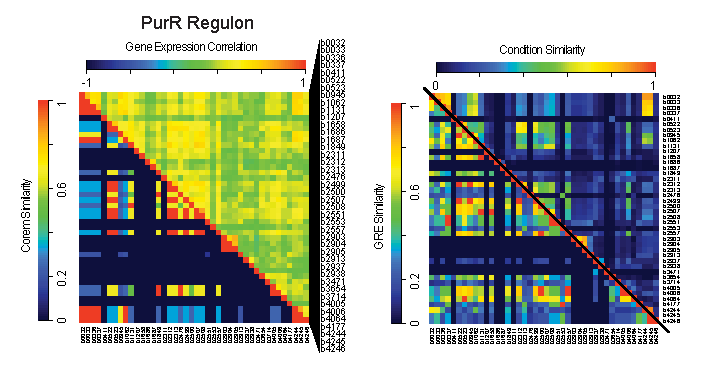
\includegraphics[width=\textwidth]{figures/purR_heatmap}
 	\caption[Corems model the mechanistic basis for conditional subdivision of the PurR regulon, \textit{E. coli.}]{(Left) Corems identify the most highly correlated subgroupings of genes in PurR regulon. Gene expression correlation across all experiments (upper triangle) compared to similarity of corem membership (lower-triangle, Jaccard index) for genes of the PurR regulon (gene identifiers expanded to right). (Right) Similarity of regulated conditions (upper triangle, Jaccard index) and GREs com- position for these genes (bottom triangle, Jaccard index). Consistent patterns of conditional-activity and GRE composition in their promoter regions further supports subdivision of PurR genes into separate corems. Gene order is same as left.
}
    \label{fig:purR_heatmap}
\end{figure}

\begin{figure}[h!]
    \centering
    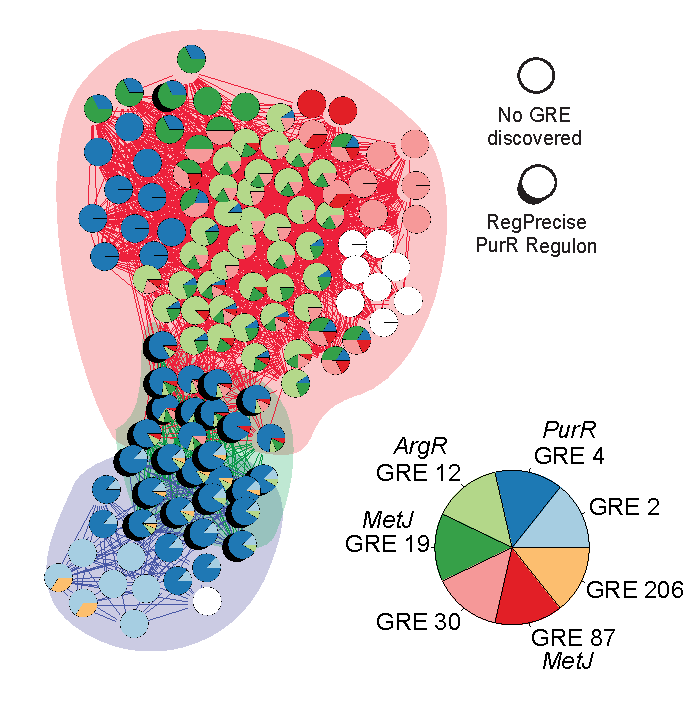
\includegraphics[width=0.75\textwidth]{figures/purR_network}
 	\caption[Corems integrate diverse regulatory mechanisms, \textit{E. coli}]{Network representation for three corems described in Figure \ref{fig:egrin2:4:A}. Genes are represented by circles. Edge colors and colored region behind the network indicate corem membership. Pie charts reflect GRE composition of each gene (see Figure \ref{fig:corem_gres}). Key for pie charts at bottom. GRE-TF matches are indicated. Shading behind nodes denotes PurR regulon genes. At least 7 different mechanisms regulate the expression of these genes.
}
    \label{fig:purR_network}
\end{figure}

\begin{figure}[h!]
    \centering
    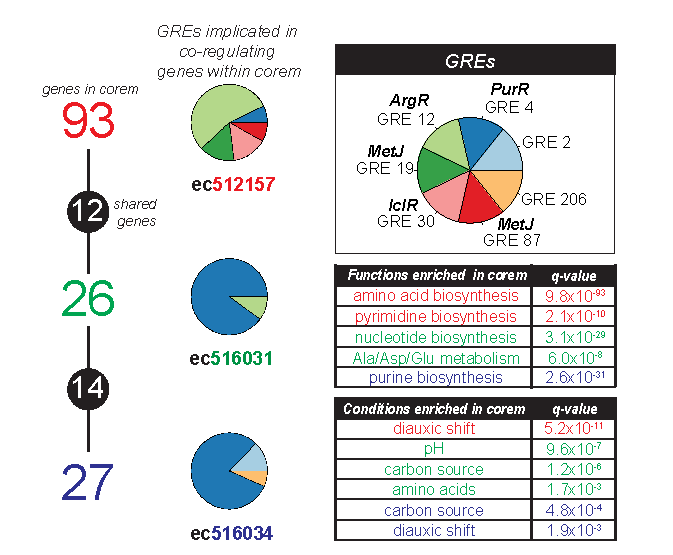
\includegraphics[width=0.65\textwidth]{figures/egrin2_ecoli_1}
 	\caption[Condition-specific subdivision and coordination of the nucleotide biosynthesis pathway, \eco: functional segregation across corems]{Genes of nucleotide biosynthesis are distributed in overlapping combinations across three \eco corems: purine (ec516034 –“purine corem”), pyrimidine (ec512157–“pyrimidine corem”), or both pathways (ec516031 –“nucleotide corem”). (Left) Gene membership and overlap for the three corems as in Figure \ref{fig:egrin2:3:B}. Pie charts indicate average GRE composition across all gene promoters in each corem (see Figure \ref{fig:corem_gres} for detail). (Top-Right Inset) GRE key for pie charts. Matches to TFs in RegulonDB noted above the GRE name. (Bottom-Right) Tables list enriched gene functions \cite{dennis_david:_2003} and environmental conditions for each of the corems (see Chapter \ref{chap:2}). 
}
    \label{fig:egrin2:4:A}
\end{figure}

\begin{figure}[h!]
    \centering
    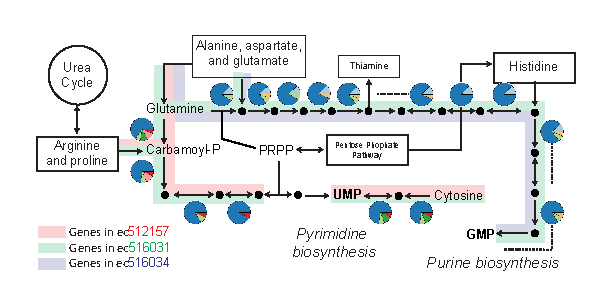
\includegraphics[width=0.8\textwidth]{figures/egrin2_ecoli_2}
 	\caption[Corems segment the nucleotide biosynthesis pathway, \eco]{A portion of the nucleotide biosynthetic pathways, near the branch point dividing purine (top) and pyrimidine (bottom) biosynthesis. Pie charts represent GRE composition in each gene promoter (Key in Figure \ref{fig:egrin2:4:A}). Operons denoted by dashed lines, with only the leader gene’s promoter architecture shown.
}
    \label{fig:egrin2:4:B}
\end{figure}

\begin{figure}[h!]
    \centering
    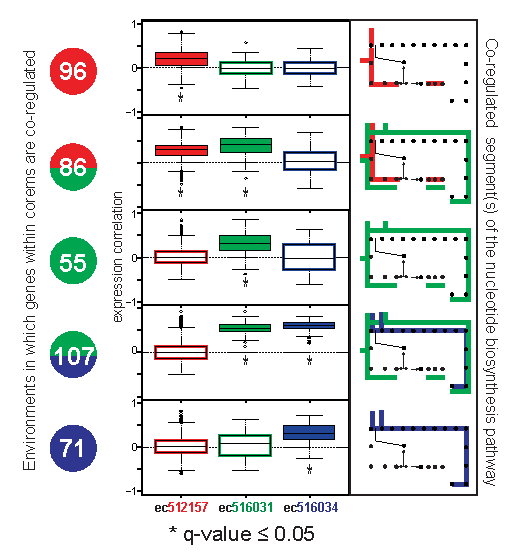
\includegraphics[width=0.6\textwidth]{figures/egrin2_ecoli_3}
 	\caption[Differential co-expression across the nucleotide biosynthesis pathway, \eco ]{Condition-specific co-expression of genes across the three corems. (Right) The active segments of nucleotide biosynthesis (as in Figure \ref{fig:egrin2:4:B}) are color-matched to corems. (Center) Box plots plots show distributions of expression correlations between genes within each corem in relevant environmental conditions, when they are predicted to be co-regulated. Color fill and asterisks indicate corems with significantly low relative standard deviation (RSD; |σ/μ|; FDR ≤ 0.05). (Left) Colored circles indicate when genes within which corem(s) are predicted to be co-regulated (color) under how many conditions (number). 
}
    \label{fig:egrin2:4:C}
\end{figure}

\begin{figure}[h!]
    \centering
    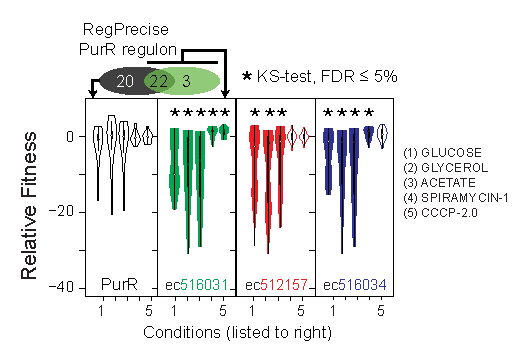
\includegraphics[width=0.8\textwidth]{figures/egrin2_ecoli_4}
 	\caption[Condition-specific fitness contributions across nucleotide biosynthesis pathway predicted by corems, \eco]{Distributions of relative fitness values for gene deletions in the three corems, as well as 20 of the 42 PurR regulon genes not modeled by ec516031 (black) across 5 representative conditions (condition identifiers listed to right, additional conditions in Figure \ref{fig:purR_corem_fitness_specific}). Asterisks denote conditions in which the distribution of fitness values is statistically significant (relative to the distribution of fitness values for all genes in that condition).
}
    \label{fig:egrin2:4:D}
\end{figure}

\begin{figure}[h!]
    \centering
    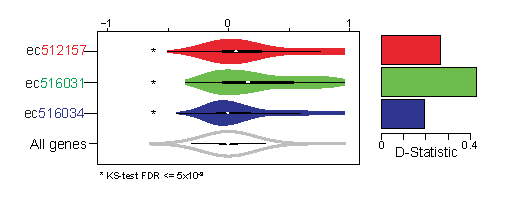
\includegraphics[width=0.8\textwidth]{figures/purR_corem_fitness}
 	\caption[Genes from corems related to nucleotide biosynthesis have highly similar fitness effects when they are deleted]{(Left) Violin plot shows distribution of all fitness correlations for genes in three nucleotide biosynthesis-associated corems compared to all genes in the data set. (Right) KS D-Statistic relates to enrichment for highly correlated gene-gene fitness associations in the corems. All three corems enrich for similar fitness effects (KS FDR $<$ 5 × $10^{−9}$)
}
    \label{fig:purR_corem_fitness}
\end{figure}

\begin{figure}[h!]
    \centering
    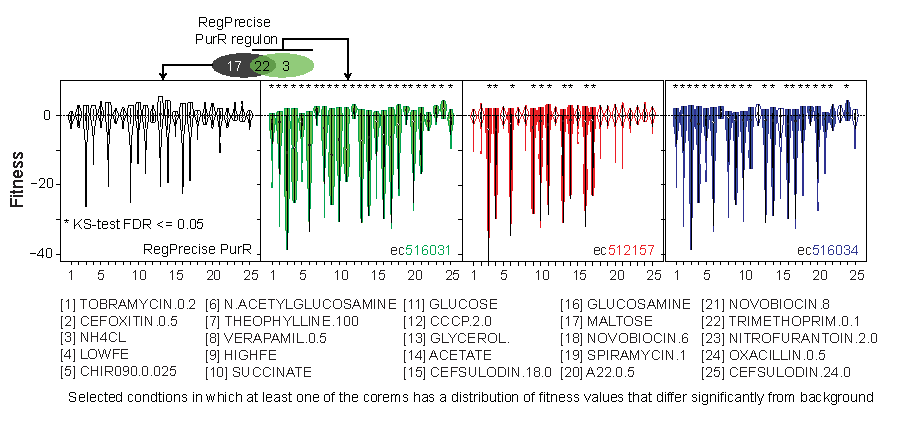
\includegraphics[width=0.8\textwidth]{figures/purR_corem_fitness_specific}
 	\caption[Corems model fitness effects that occur in specific environments]{Violin plots show distribution of relative fitness among corems across conditions (negative values indicate lower fitness relative to WT). Brief condition descriptions are displayed below. Shading within the violin plot indicates that the distribution of fitness values is significantly in that condition (KS-test FDR $\leq$ 0.05). Fitness values for the subset of genes from the PurR regulon that do not occur in ec516031 are displayed to the left. These genes do not have significant fitness effects in any of the environments tested.
}
    \label{fig:purR_corem_fitness_specific}
\end{figure}

This example highlights two important features of \egrine~ and corems. First, \egrine~ can distinguish co-regulation by independent, similarly-acting TFs, even though their targets are co-expressed. Further, corems group together genes that are functionally-related even though their co-regulation is mediated by different mechanisms, demonstrating how conditional TF-influences in a GRN coordinate transcription of genes from different regulons whose deletions have highly correlated fitness consequences (Table \ref{tab:table1}). Genes of the pyrimidine corem, for example, are co-regulated by as many as five TFs. Even though promoters of each of the genes in this corem contain distinct compositions of GREs (Figure \ref{fig:purR_network}, Tables S9-S10), their expression is highly coordinated across a broad range of conditions. Interestingly and counter to our expectation, transcript level changes of the similarly acting TFs are not highly correlated. Instead, we discovered correlated changes in the concentrations of effector molecules, which allosterically regulate the activities of these TFs, suggesting that coordinate regulation of genes in the pyrimidine corem is a direct consequence of metabolic dynamics (Figure \ref{fig:purR_effector}; \cite{ishii_multiple_2007}).

\begin{figure}[h!]
    \centering
    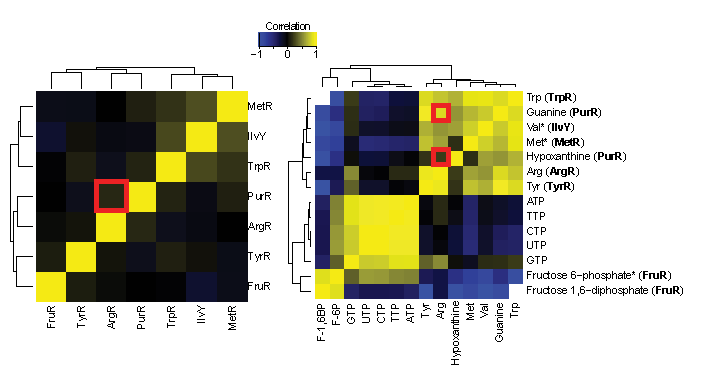
\includegraphics[width=0.8\textwidth]{figures/purR_effector}
 	\caption[Metabolite correlations may explain co-regulation within metabolically-linked corems]{(Left) Expression correlation for TFs associated with three corems described in the text (ec516031,ec512157,ec516034). (Right) Correlation allosteric regulators for these TFs. TF regulated by each biomolecule listed in parentheses. Red boxes indicate PurR-ArgR and their corresponding effector molecules. Data from \cite{ishii_multiple_2007}.
}
    \label{fig:purR_effector}
\end{figure}

% Table 1
% Table generated by Excel2LaTeX from sheet 'highfit_regprecise_sub.txt'
\begin{table}[htbp]
  \centering
  \caption{Corems group together genes from different regulons with highly correlated fitness effects}
  \resizebox{\columnwidth}{!}{%
    \begin{tabular}{c c p{5cm} c c c}
    \toprule
    \multicolumn{1}{c}{\textbf{Gene 1}} & \multicolumn{1}{c}{\textbf{Gene 2}} & \multicolumn{1}{c}{\textbf{Fitness correlation}} & \multicolumn{1}{c}{\textbf{Regulon Gene 1}} & \multicolumn{1}{c}{\textbf{Regulon Gene 2}} & \multicolumn{1}{c}{\textbf{Corems}} \\
    \midrule
    \multicolumn{1}{c}{\textit{b3774}} & \multicolumn{1}{c}{\textit{b3959}} & \multicolumn{1}{c}{0.959012} & \multicolumn{1}{c}{IlvY} & \multicolumn{1}{c}{ArgR} & \multicolumn{1}{c}{512157} \\
    \multicolumn{1}{c}{\textit{b2913}} & \multicolumn{1}{c}{\textit{b3829}} & \multicolumn{1}{c}{0.938764} & \multicolumn{1}{c}{PurR} & \multicolumn{1}{c}{MetR} & \multicolumn{1}{c}{512157} \\
    \multicolumn{1}{c}{\textit{b3829}} & \multicolumn{1}{c}{\textit{b3959}} & \multicolumn{1}{c}{0.934393} & \multicolumn{1}{c}{MetR} & \multicolumn{1}{c}{ArgR} & \multicolumn{1}{c}{512157;554056} \\
    \multicolumn{1}{c}{\textit{b2913}} & \multicolumn{1}{c}{\textit{b3941}} & \multicolumn{1}{c}{0.932025} & \multicolumn{1}{c}{PurR} & \multicolumn{1}{c}{MetR} & \multicolumn{1}{c}{512157} \\
    \multicolumn{1}{c}{\textit{b3957}} & \multicolumn{1}{c}{\textit{b3941}} & \multicolumn{1}{c}{0.931565} & \multicolumn{1}{c}{ArgR} & \multicolumn{1}{c}{MetR} & \multicolumn{1}{c}{512157;554056} \\
    \multicolumn{1}{c}{\textit{b3172}} & \multicolumn{1}{c}{\textit{b3829}} & \multicolumn{1}{c}{0.930382} & \multicolumn{1}{c}{ArgR} & \multicolumn{1}{c}{MetR} & \multicolumn{1}{c}{512157;554056} \\
    \multicolumn{1}{c}{\textit{b2913}} & \multicolumn{1}{c}{\textit{b3774}} & \multicolumn{1}{c}{0.927776} & \multicolumn{1}{c}{PurR} & \multicolumn{1}{c}{IlvY} & \multicolumn{1}{c}{512157;512477} \\
    \multicolumn{1}{c}{\textit{b3941}} & \multicolumn{1}{c}{\textit{b3774}} & \multicolumn{1}{c}{0.927251} & \multicolumn{1}{c}{MetR} & \multicolumn{1}{c}{IlvY} & \multicolumn{1}{c}{512157} \\
    \multicolumn{1}{c}{\textit{b3960}} & \multicolumn{1}{c}{\textit{b3941}} & \multicolumn{1}{c}{0.921375} & \multicolumn{1}{c}{ArgR} & \multicolumn{1}{c}{MetR} & \multicolumn{1}{c}{512157;554056} \\
    \multicolumn{1}{c}{\textit{b3941}} & \multicolumn{1}{c}{\textit{b3959}} & \multicolumn{1}{c}{0.921282} & \multicolumn{1}{c}{MetR} & \multicolumn{1}{c}{ArgR} & \multicolumn{1}{c}{512157;554056} \\
    \bottomrule
    \end{tabular}%
    }
  \label{tab:table1}%
\end{table}%


Second, \egrine~ predicts that not all locations that match to the same GRE are functionally equivalent in all environments. Accordingly, using corems we can discern and explain why genes regulated by the same TF exhibit different expression patterns in certain environments. For example, out of the 42 PurR-regulated genes (assigned by RegPrecise), expression changes of the 14 that are grouped into the purine corem are better correlated with each other and genes of this corem than they are to the portion of the PurR regulon that was left out (t-test, pval $< 2.2\times10^{-16}$, Figure \ref{fig:egrin2:5:A}). Consistent with this observation, PurR is predicted to play a variable role in regulation of genes across the three corems (from being highly important for the nucleotide corem, to being marginally important for the pyrimidine corem, Figure \ref{fig:egrin2:4:A}). We hypothesized that the degree to which PurR is implicated in regulating genes within each corem is a good predictor of target-specific expression consequences of knocking out this TF. To test this hypothesis we analyzed global transcriptional changes in both wild type (WT) and $\Delta$purR deletion strains of \eco grown in the presence of adenine \cite{cho_purr_2011}. These data were obtained from experiments that were not included in construction of the \egrine~ model. Specifically, we calculated the relative standard deviation (a measure of co-regulation) for every PurR-associated corem in each of the two strains. As expected, genes in all three corems described above were co-regulated in the WT strain (FDR $<$ 0.05, Figure \ref{fig:egrin2:5:B}). Strikingly consistent with \egrine~predictions, the degree of dysregulation of genes within each of the three corems in the $\Delta$purR strain was proportional to the predicted magnitude of PurR influence. Maximal dysregulation of genes in the nucleotide corem and the purine corem, for example, was consistent with the predicted role of PurR as the primary regulator of genes in these corems (Figure fig:egrin2:5:C). Notably, the degree of disruption observed in these two corems surpasses that of the entire PurR regulon, suggesting that in the presence of adenine, PurR regulates only a subset of its target genes. These results illustrate how the concept of a corem captures the context in which TF binding to a GRE is functional, not just that the potential for TF-GRE interaction exists, which is how a regulon is defined.

\begin{figure}[h!]
    \centering
    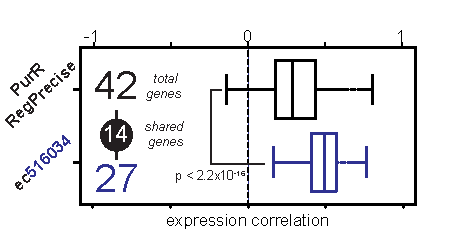
\includegraphics[width=0.8\textwidth]{figures/egrin2_ecoli_expression_cor}
 	\caption[Transcriptional evidence for subdivision of regulons by corems]{Distributions of pairwise expression correlations among all genes in the PurR regulon (RegPrecise) compared to a subset of the regulon within corem ec516034, across all environmental conditions. Also shown are the total number of genes in each group, and the number of shared genes. The two distributions are significantly different (Welch Two Sample t-test, p $< 2.2^{-16}$).
}
    \label{fig:egrin2:5:A}
\end{figure}

\begin{figure}[h!]
    \centering
    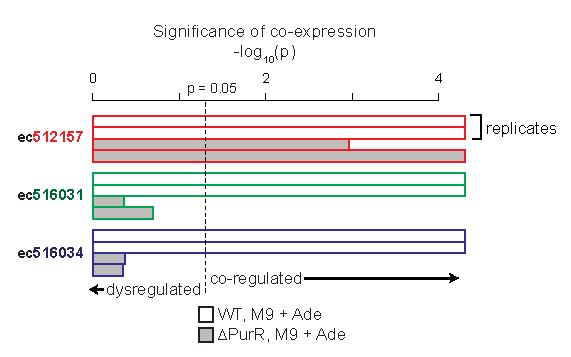
\includegraphics[width=0.8\textwidth]{figures/egrin2_ecoli_ko_expression}
 	\caption[Corems with predicted influence from PurR (GRE \#4) are disrupted in $\Delta$purR mutant]{RSD of transcript level changes (resampled -log10(pval)) for the three corems in Figure \ref{fig:egrin2:4:A} in WT and $\Delta$purR strains of \eco (both grown with adenine). The dashed line delineates significant co-expression (p = 0.05). 
}
    \label{fig:egrin2:5:B}
\end{figure}

\begin{figure}[h!]
    \centering
    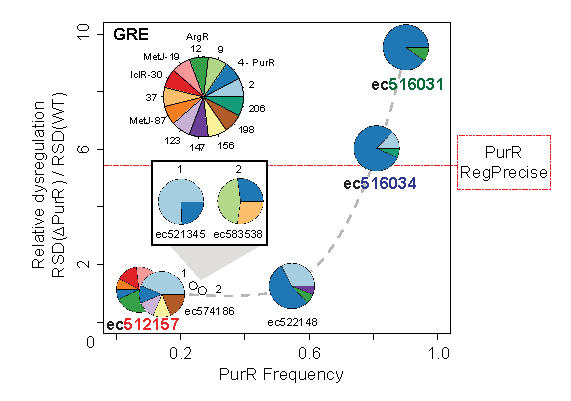
\includegraphics[width=0.8\textwidth]{figures/egrin2_ecoli_purR_predictive}
 	\caption[GRE \#4 influence predicts which corems are disrupted in $\Delta$purR mutant]{Relative RSD ($\Delta$purR/WT) for all seven GRE \#4-associated corems plotted as a function of the frequency with which GRE \#4 (PurR) is discovered within these corems. Composition of GREs discovered within each corem are shown as pie charts (as in Figure \ref{fig:egrin2:4:A}), with key in inset, top-right. Relative RSD of the RegPrecise PurR regulon is shown for reference (dotted horizontal line).
}
    \label{fig:egrin2:5:C}
\end{figure}

\section{Discussion}

\egrine~explains how microbes tailor transcriptional responses to varied environments by linking the genome-wide distribution of GREs to their organization and conditional activities within each promoter. The integrative model reveals the mechanisms by which microbes reuse genes in varying combinations to operationally link disparate processes and regulate flux through metabolic pathways. We have provided extensive validations for predictions made by \egrine~for a bacterium and an archaeon (Table 2). In addition, we also performed new experiments to validate a model prediction that widespread transcriptional activity at non-canonical locations within genes and operons was partly responsible for complex modulation of the \eco transcriptome during growth in rich media.  

Corems represent a fundamental organizing principle of GRNs that captures fitness-relevant associations among genes, forging a link between the environment-dependent dynamics of transcriptional control and phenotype. The conditional associations among genes across corems reflect the underlying structure of coupled changes in environmental factors, such as correlated changes in effector molecules. Comparative analyses of \egrine~models, therefore, could reveal the corems associated with unique and shared environmental structures that distinguish ecotypes of the same species.

\egrine~will provide context-relevant engineering strategies for synthetic biology because it models environment-dependent coordination of diverse regulatory mechanisms operating across the entire genome, including non-canonical locations. By teasing apart regulatory mechanisms that have indistinguishable outputs in certain environments, \egrine~offers multiple strategies for introducing new genes into the GRN. For instance, there are at least five distinct mechanisms responsible for co-regulating nearly 100 genes in the pyrimidine corem in \eco. This corem coordinates genes from various segments of amino acid biosynthesis pathways, including arginine biosynthesis, as well as the pentose phosphate pathway to synchronize inputs into nucleotide biosynthesis. The conditional grouping of genes into the pyrimidine corem explains the previous observation that genes of arginine biosynthesis are repressed upon adenine addition \cite{cho_purr_2011}. \egrine~predicts that this coordination of nucleotide and arginine biosynthesis is accomplished by an equivalency of PurR and ArgR activities under these conditions (possibly due to correlated changes in effector molecules), rather than by direct regulation of arginine biosynthesis genes by PurR. Not surprisingly, subsets of genes within this corem belong to alternate regulatory programs (corems) under different environmental contexts. Thus, depending on the objective, we can select a reengineering strategy from a library of mechanisms that already exist within the GRN of an organism. Future work to translate the \egrine~model into the language of synthetic biology will enable systems-level reengineering of an organism.
